\documentclass[10pt]{beamer}
\usepackage{templates/beamerthemekit}

\usepackage{amsmath,amssymb,amsbsy}
\usepackage{subcaption}
\usepackage{caption}
\captionsetup[figure]{labelformat=empty}
\usepackage{graphicx}
\usepackage{adjustbox}
\usepackage{amsfonts}
\usepackage{array}        
\usepackage{topcapt}          % To use captions above the tables
\usepackage{tikz}
\usepackage{booktabs}
\usepackage{multirow}
\usepackage{mathtools}
\usepackage{xcolor}
\usepackage{tikz}
\usepackage{framed}  

\usetikzlibrary{shapes,arrows}
\usetikzlibrary{positioning}
\tikzstyle{decision} = [diamond, draw, fill=blue!20, 
text width=4.5em, text badly centered, node distance=3cm, inner sep=0pt]
\tikzstyle{block} = [rectangle, draw, fill=blue!20, 
text width=5em, text centered, rounded corners, minimum height=4em]
\tikzstyle{line} = [draw, -latex']
\tikzstyle{cloud} = [draw, ellipse,fill=red!20, node distance=3cm,
minimum height=2em]


\graphicspath{{./figs/}}

\newcommand{\av}[1]{\overline{#1}}
\newcommand{\avef}[1]{\langle #1 \rangle_A}
\renewcommand{\vec}[1]{\mathbf{#1}}
\newcommand{\wav}[1]{\langle #1 \rangle_w}
\newcommand{\Rey}{\text{Re}}
\newcommand{\light}[1]{\textcolor{gray}{#1}}

\definecolor{dodgerblue}{HTML}{1E90FF}
\definecolor{crimson}{HTML}{DC143C}
\definecolor{seagreen}{HTML}{2E8B57}

\titleimage{matrix_struct}

\title{Parallelism study of iterative linear solvers using Regent and CUDA}

\subtitle{EE382N-20 - Parallelism and Locality}
\date{May 17, 2019}
\author{Grant Guglielmo, Ashwin Krishnan, \\Manish Ravula, Nicholas Deak}
%\institute{Clean Combustion Research Center} 
%\institute{$^1$ The University of Texas at Austin, Austin, TX, USA}

%\usepackage[bibstyle=authoryear, citestyle=authoryear-comp]{biblatex}
\usepackage{natbib}
%\addbibresource{biblio.bib}
%\bibhang1em

%(add pics)
%(add table for dimensions slide)

\begin{document}
\selectlanguage{english}

\begin{frame}
\titlepage
\end{frame}


\begin{frame}{Presentation Outline}
	
	\begin{itemize}
		
		\item Problem motivation and background
		\bigskip
		
		\item CUDA implementation results 
		\bigskip
		
		\item Regent implementation results, and comparison to CPU performance
		\bigskip
		
		\item Results discussion and conclusions
		
	\end{itemize}
	
\end{frame}

\begin{frame}{Sparse Linear Systems}
	
	\begin{columns}
		\column{0.6\textwidth}
		\begin{itemize}
			\item Linear systems arise naturally when discretizing PDEs to solve numerically	
			
			\item Systems are usually quite sparse in nature, and follow certain patterns
			
			\item Direct solvers are generally of complexity O($n^{3}$), which can be cost prohibitive for large systems
			
			\item Additionally, direct solve storage requirements also become an issue, as factors of a sparse matrix are generally non-sparse
			\pause
			
			\item \textbf{Iterative solvers are crucial to handling these types of problems}
			
		\end{itemize}
		\column{0.4\textwidth}
			\begin{figure}[H]
			\centering
			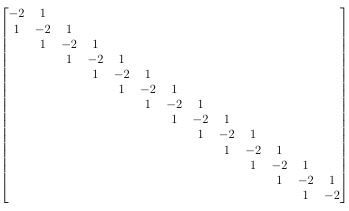
\includegraphics[scale=0.60]{case1.jpg}
			\label{fig:case1} 
		\end{figure}
		\begin{figure}[H]
			\centering
			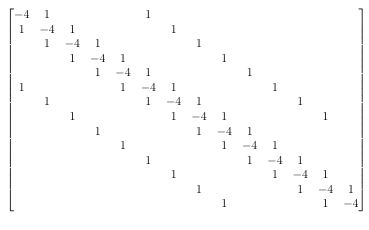
\includegraphics[scale=0.60]{case2.jpg}
			\label{fig:case2} 
		\end{figure}
		
	\end{columns}	
\end{frame}

\begin{frame}{Conjugate Gradient Method}
	
	\begin{columns}
	\column{0.6\textwidth}
	\begin{itemize}
		\item Common iterative method used for solving sparse linear systems	
		
		\item Designed to work on SPD matrices, but can be expanded to work on more general cases
		
		\item Can be thought of as solving a minimization problem $q(x) = \frac{1}{2} \cdot Ax - x \cdot b$
		
		\item search directions and an optimal step size are chosen at each iteration, until $|| Ax - b ||_{2}$ falls below some threshold
		
	\end{itemize}
	\column{0.4\textwidth}
	\begin{figure}[H]
		\centering
		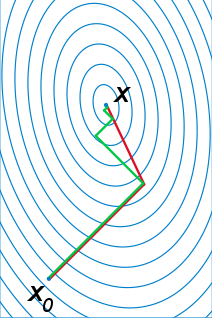
\includegraphics[scale=0.50]{CG_vis.png}
		\label{fig:CG_vis} 
	\end{figure}
	\end{columns}		
	
\end{frame}

\begin{frame}{CUDA Results}
	
\end{frame}


\begin{frame}{Regent Implementation}
	
\end{frame}


\begin{frame}{Conclusions}
	
\end{frame}

\end{document}